\documentclass{Preport}

\usepackage{placeins}
\usepackage{hyperref}
\usepackage{amsmath}
\hypersetup{
    colorlinks=true,
}

\exname{万用表的设计} %实验名称
\instructor{谭艾林} %指导教师
\class{github} %班级
\name{MJ} %姓名
\stuid{2025} %学号

\nyear{2025} %年
\nmonth{12} %月
\nday{22} %日
\nweekday{一} %星期几

\begin{document}
\setcounter{page}{0}
\makecover

\section{预习报告（10分）}
\subsection{实验综述（5分）}

万用表主要由直流电流计及若干电阻构成，本实验要设计指针式万用表，主要是由磁电式电流计以及一系列电阻组成。
其中电流计有两个主要参数，用 $I_g$ 表示电流计允许通过的最大电流， 用 $R_g$ 表示电流计线圈的电阻。

要改装量程为 $I$ 的电流表，需要在电流计两端并联一个分流电阻，阻值满足 $R_s = \frac{R_g I_g}{I-I_g}$ ，
选取不同的电阻即可构成不同量程的电流表。

当使用量程为 $I_g = 1 mA$ 的电流计改装为有 $5 mA$ 和 $10 mA$ 两个量程的电流表时，设计如图：
\begin{figure}[htpb!]
    \centering
    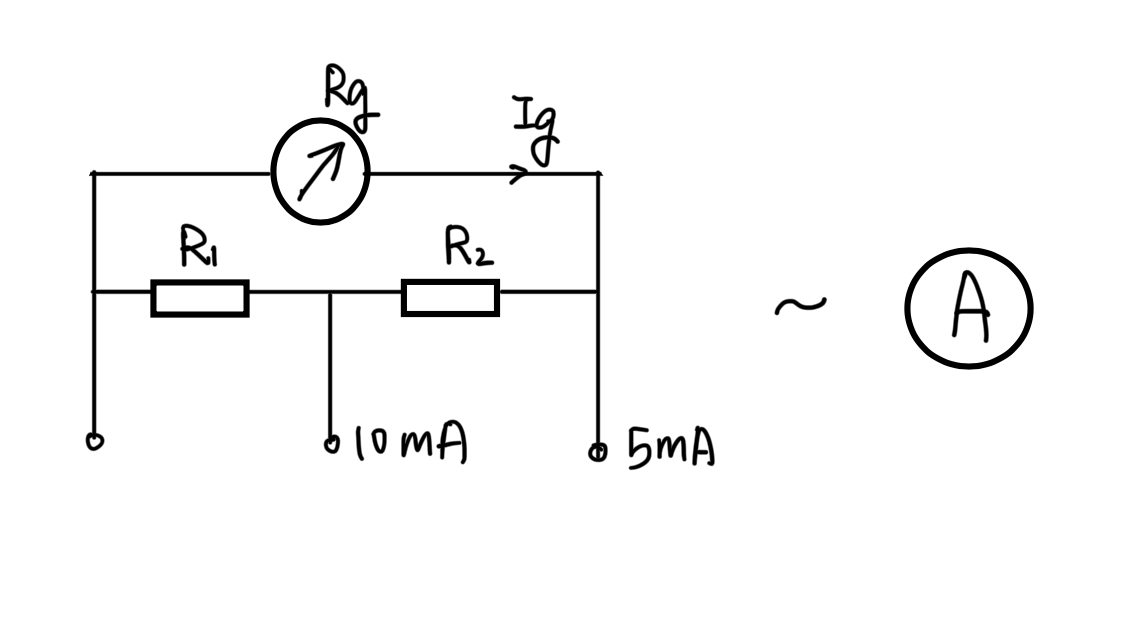
\includegraphics[width = 0.35\textwidth]{fig1.jpg}
\end{figure}

其中并联的电阻阻值满足：

\[
\begin{cases}
    (R_1 + R_2)(5 - I_g) = R_g I_g \\
    (R_2 + R_g) I_g = R_1 (10 - I_g)
\end{cases}
\]

然后使用标准安培表校正改装后的电流表，并分析误差，如图：
\begin{figure}[htpb!]
    \centering
    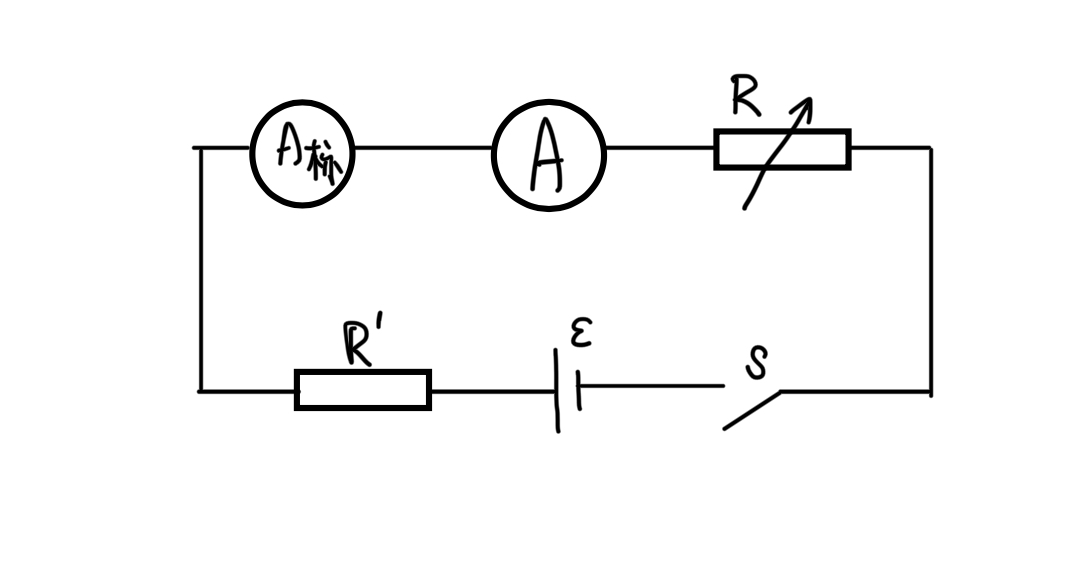
\includegraphics[width = 0.3\textwidth]{fig2.jpg}
\end{figure}

其中 $A_{\text{标}}$ 为标准安培表， $A$ 为改装电流表， $R$ 为可调节电阻， $R'$ 为限流保护电阻， $\epsilon$ 为直流电源。

要改装量程为 $U$ 的电压表，使用改装后的电流计并串联一个分压电阻，阻值满足 $R_x = \frac{U}{I_g'} - R_g'$ ，
其中 $R_g'$ 为电流计等效内阻， $I_g'$ 为电流计等效量程。

当要改装为有 $5V$ 和 $10V$ 两个量程的电压表时，设计如图：
\begin{figure}[htpb!]
    \centering
    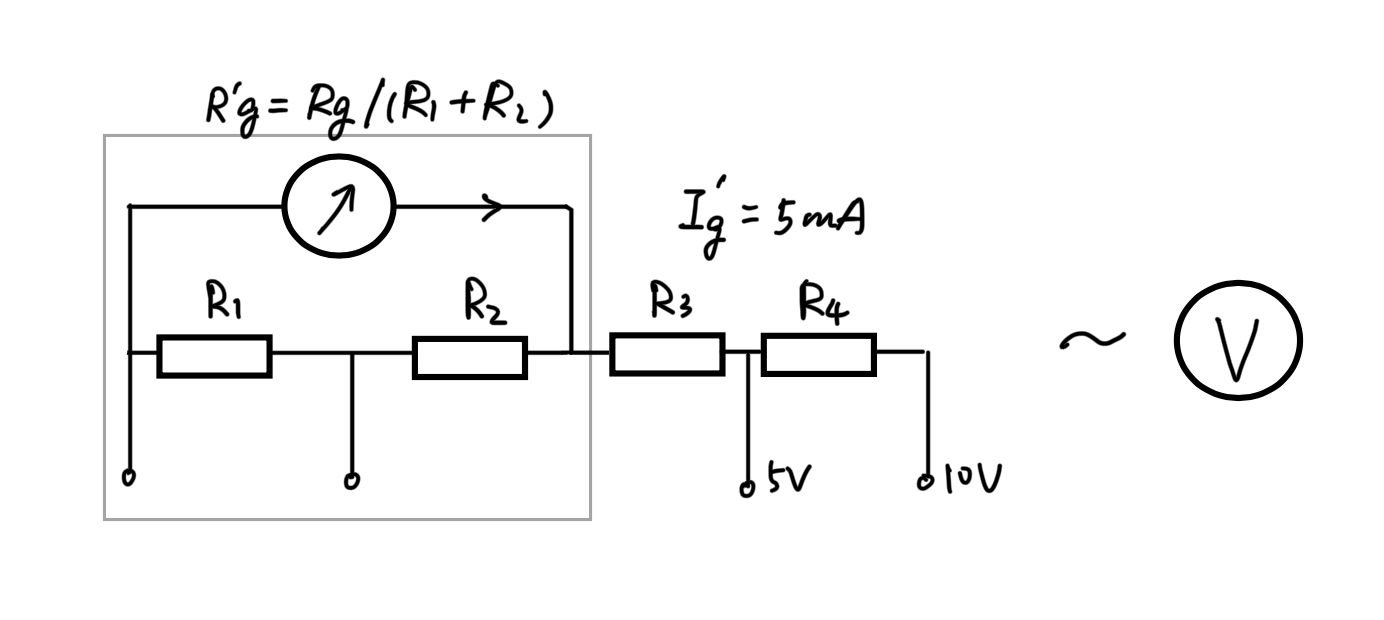
\includegraphics[width = 0.4\textwidth]{fig3.jpg}
\end{figure}

其中串联的电阻阻值满足：

\[
\begin{cases}
    I_g' (R_g' + R_3) = U_1 \\
    I_g' (R_g' + R_3 + R_4) = U_2     
\end{cases}
\]

然后使用标准伏特表校正改装后的电压表，并分析误差，如图：
\begin{figure}[htpb!]
    \centering
    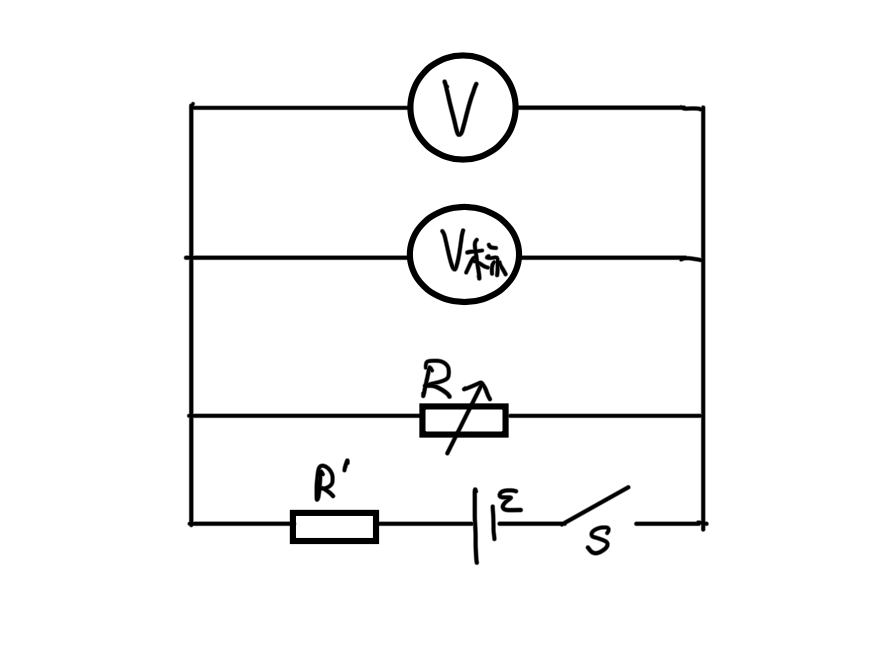
\includegraphics[width = 0.3\textwidth]{fig4.jpg}
\end{figure}

其中 $V_{\text{标}}$ 为标准伏特表， $v$ 为改装电压表， $R$ 为可调节电阻， $R'$ 为限流保护电阻， $\epsilon$ 为直流电源。


改装欧姆表时，需要短接 $a、b$ 两端并调节电阻 $R$ 使得电流计满刻度，此时满足 $\epsilon = I_0 (R_g' + R')$ ；
接入待测电阻后，回路满足 $\epsilon = I_x (R_g' + R' + R_x)$ 。当 $R_x = R_g + R'$ 时有 $I_x = \frac{I_0}{2}$ ，
此时电表指针指向刻度线中点，电阻 $R_x$ 称为欧姆表中值电阻，据此可以用电流计测量不同的电阻阻值。

此外由于电源电池非恒定，所以需要在电路中串联一电位器 $R_6$ 作零欧姆调整，如图：
\begin{figure}[htpb!]
    \centering
    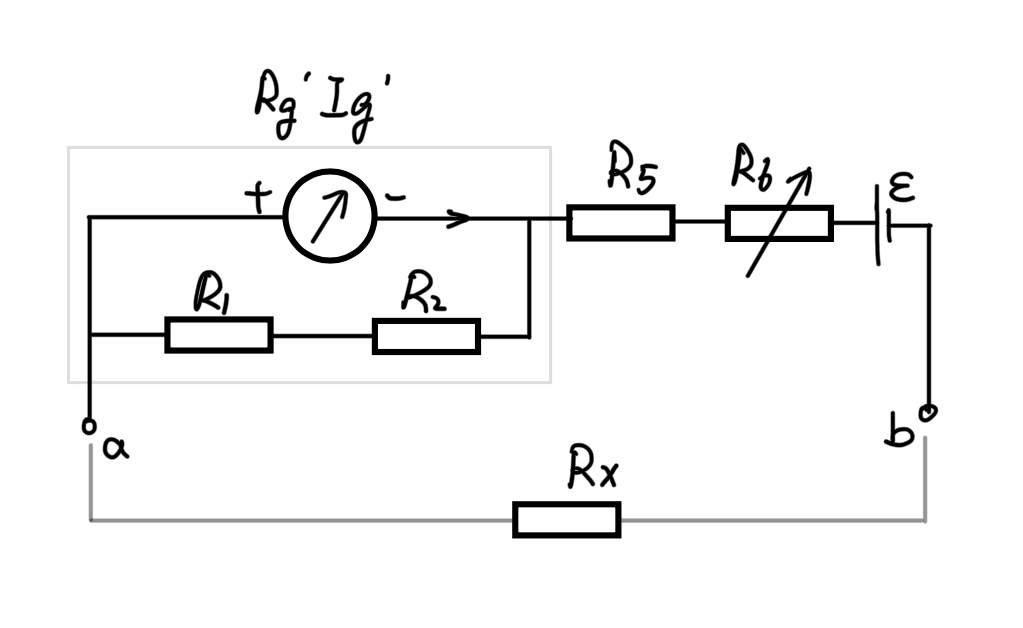
\includegraphics[width = 0.35\textwidth]{fig5.jpg}
\end{figure}

\subsection{实验重点（3分）}

本实验的重点在于了解指针式万用表的结构和测量电流、电压和电阻的基本原理，并掌握使用磁电式电流计改装多量程电流表、电压表和欧姆表的方法；
同时学习如何通过标准电表和可调节电阻校准万用表。

\subsection{实验难点（2分）}

本实验的难点在于准确计算和选取分流或分压电阻，因为有偏差会影响电表量程准确性；
改装后必须校准电表，控制电流或者电压稳定；在改装欧姆表时由于刻度非线性，设计要求较高；
此外需要考虑电流计内阻对电表的影响。

$\quad$

\input{注意事项}
\end{document}
